\documentclass[a4paper,12pt]{report} 
\usepackage[utf8x]{inputenc}
\usepackage[french]{babel}
\usepackage{mathtools}
\usepackage{amsmath, amssymb, amsfonts}
\usepackage{textcomp}
\usepackage[nointegrals]{wasysym}			% Collection de symboles mathématiques
\usepackage{multicol}					% Pour utiliser \hfill
\usepackage{ifthen}
\usepackage{tabularx}	 				% Gestion avancée des tableaux
%\usepackage{cleveref}

\usepackage{enumitem}
\usepackage{wrapfig}
%\usepackage[squaren]{SIunits}
%\usepackage[T1]{fontenc}				% Indispendable, présent dans tous les codes exemples
\usepackage[linkcolor=Indigo,colorlinks=true, citecolor=SaddleBrown, urlcolor=MidnightBlue]{hyperref} 	% Hyper ref
\usepackage{listings}					% Pour citer du code
\usepackage[justification=centering]{caption}
\usepackage{sistyle} 
\usepackage{numprint}
\usepackage{wrapfig}
\usepackage{cite}	
\usepackage{url} 					% Pour citer les sites internet dans la
%\usepackage{cleveref}
\usepackage{setspace}

\usepackage{graphicx}		 			% Inclusion des figures
\graphicspath{{./pic/}}
\usepackage[svgnames]{xcolor}			%https://www.latextemplates.com/svgnames-colors

%%% Commandes utiles définies
\newcommand{\argmin}{\mathop{\mathrm{argmin}}}

\newcommand{\bepar}[1]{
	\left( #1 \right)  
}

\newcommand{\becro}[1]{
	\left[ #1 \right]  
}

\newcommand{\rbk}[1]{\color{red}\textit{#1} \color{black}  
}

\usepackage{listings}					% Pour citer du code
%%%%%%%%%%%%%%%%%%%
%%% Élément pour citer des codes %%%
\lstset{
language=Python,
basicstyle=\ttfamily\bfseries\small, %
identifierstyle=\bfseries\color{black}, %
keywordstyle=\color{blue}, %
stringstyle=\color{black!90}, %
commentstyle=\it\color{black!70}, %
columns=flexible, %
tabsize=4, %
extendedchars=true, %
showspaces=false, %
showstringspaces=false, % %
numberstyle=\small, %
breaklines=true, %
breakautoindent=true, %
captionpos=b,
otherkeywords={cross_val_score},
keywords=[0]{cv},
keywordstyle=[0]{\color{red}},
}
%%%%%%%%%%%%%%%%%%%%%
\title{\navy \textbf{Notes bibliographiques : \\ Utilisation de ML pour la turbulence} \color{black}}%%%%%%%%%%%%%%%%%%%%
\date{}
%\usepackage{multicol}
%\usepackage{etoolbox}
%\patchcmd{\thebibliography}{\section*{\refname}}
%    {\begin{multicols}{2}[\section*{\refname}]}{}{}
%\patchcmd{\endthebibliography}{\endlist}{\endlist\end{multicols}}{}{}
\usepackage[authoryear]{natbib}

\usepackage{geometry}
\geometry{hmargin=2cm, vmargin=2cm}

%%%%%%%%%%%%%%%%%%%%
%%% Couleurs %%%
\xdefinecolor{brick}{named}{DarkRed}
\xdefinecolor{navy}{named}{Navy}
\xdefinecolor{midblue}{named}{MidnightBlue}
\xdefinecolor{dsb}{named}{DarkSlateGray}
\xdefinecolor{dgreen}{named}{DarkGreen}

%%% 	Raccourcis 	%%%
\newcommand{\keps}{$k-\varepsilon$}
\newcommand\bk{\color{black}}
\newcommand\brick{\color{brick}}
\newcommand\navy{\color{navy}}
\newcommand\midblue{\color{midblue}}
\newcommand\dsb{\color{dsb}}
\newcommand{\dgreen}{\color{dgreen}}
\newcommand\red{\color{red}}

%%%%%%%% Cigles
\newcommand{\rap}{par rapport}
\newcommand{\cad}{c'est-à-dire}
\newcommand{\vav}{vis-à-vis}

%%%%%%%% Autres

%%%%%%%%%%%%%%%%%%%
% Syntax: \colorboxed[<color model>]{<color specification>}{<math formula>}
\newcommand*{\colorboxed}{}
\def\colorboxed#1#{%
  \colorboxedAux{#1}%
}
\newcommand*{\colorboxedAux}[3]{%
  % #1: optional argument for color model
  % #2: color specification
  % #3: formula
  \begingroup
    \colorlet{cb@saved}{.}%
    \color#1{#2}%
    \boxed{%
      \color{cb@saved}%
      #3%
    }%
  \endgroup
}
\renewcommand{\sectionmark}[1]{\markright{#1}}
\usepackage{fancyhdr}
\pagestyle{fancy}
\lhead{\textbf{Nathaniel} \brick \textbf{\textsc{Saura}}}
\rhead{\markright}
\cfoot{\thepage}
\renewcommand{\headrulewidth}{0.4pt}

\numberwithin{equation}{section} %%%% To count the equation like Section.Number

\usepackage{accents}
\newcommand{\vect}[1]{\accentset{\Rightarrow}{#1}}

\begin{document}
\maketitle
\newcolumntype{M}[1]{>{\centering\arraybackslash}m{#1}}
\newcolumntype{N}{@{}m{0pt}@{}}

%\noindent On se base sur \textbf{\citep{ling2016machine}} qui se pose la question de comment inculquer les propriétés d'invariance lors de l'apprentissage, et de voir si le faire améliore les prédictions.
\begin{table}[!ht]
		% Center the table
		\centering
		% Table itself: here we have two columns which are centered and have lines to the left, right and in the middle: |c|c|
		\begin{tabular}{|M{.22\textwidth}|M{.72\textwidth}|N }
		\hline
		Auteur & Travaux &\\[.5cm] \hline

		\textbf{\cite{ling2015evaluation}} & Used \red Random Forests (RF) \bk to \navy predict regions of high model from uncertainty in RANS results.\bk &\\[1.5cm] \hline

		\textbf{\cite{ling2016machine}} &Use of \red RF \bk with Gini Impurity Score, max\_depth = 15  and 500 DT whose output are averaged, and \red NN\bk with sigmoid activation function. In the previous work, Ling et \textit{al.} predict the Reynolds Stress Anisotropy $\textbf{A} = \frac{1}{2k} \bar{\textbf{u} \otimes \textbf{u}} - \frac{1}{3}\textbf{Id}$ en un point à partir des images de \textbf{S} et \textbf{R} par les vecteurs d'une base d'invariants bien choisie, en tout point du domaine, ou aux points dont l'incertitude est la plus grande. Les entrées peuvent être aussi bien les invariants de la base que les 9 composantes non nulles cumulées de $\textbf{S}$ et $\textbf{R}$.&\\[4.5cm] \hline		
		
		\textbf{\cite{ling2016reynolds}} & Use of \red NN \bk embbeded with an invariant Tensor Layer element-wise mutliplied with the last HL of the Network. Use of leakyReLu act function. Trained with BPGD, the output is post-processed (see part.2, p.157). It has 8 HL, with each 30 nodes except for the last HL that has 10 nodes and $learning\_rate = 2.5 \times 10^{-7}$. Cross Validation ensures robustness of the TBNN. &\\[3.5cm]\hline		
		
		\textbf{\cite{milano2002neural}} & Used DNS results for a turbulent channel flow to train a \red NN \bk to reconstruct the \navy near wall flow \bk&\\[1.5cm] \hline
		
		\textbf{\cite{tracey2013application}} & ML algorithms (\red??\bk) to model the \navy Reynolds stress anisotopy\bk  &\\[1.5cm] \hline
		
		\textbf{\cite{tracey2015machine}} & \red NN \bk to \navy mimic the source terms from the SA turbulence model \bk &\\[1.5cm] \hline
				
		\textbf{\cite{duraisamy2015new}} & \red NN and GP \bk to \navy model intermittency in transitional turbulence \bk &\\[1.5cm] \hline 		
		
		\textbf{\cite{zhang2015machine}} & Used \red NN and GP \bk to \navy model turbulence Production in channel flow \bk &\\[1.5cm] \hline
		
		\textbf{\cite{singh2017machine}} &Use \red NN \bk to augment SA model to predict turbulent flow over airfoils (strong adverse pressure gradient). First of all use adjoint-based full field inference to infer $\beta$ the correction needed between SA and DNS or Exp. The \red NN \bk proposed here has 2 HL with 100 nodes each, using sigmoid act function. The training used BPGD minimizing an Sum Squarred Error problem.&\\[3cm] \hline 
				
		\end{tabular} 
		\vspace{0.5cm}
		
%		\caption{Tableau retraçant les études NN vs Turbulence faites auparavant 
%		\label{tab:simParameters}}
\end{table}

\pagebreak

\subsection*{\textbf{\cite{singh2017machine}} : }
\noindent L'idée de cet article peut être schématisée par la figure suivante (extraite de l'article) :

\begin{figure}[!ht]
\centering
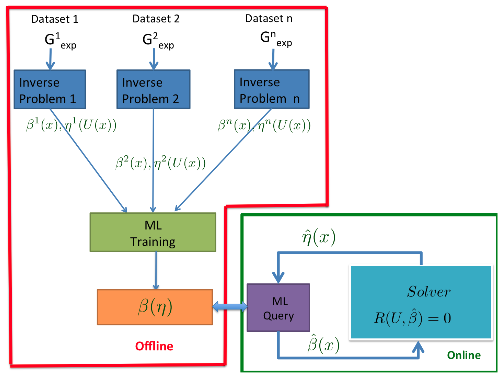
\includegraphics[scale=0.8 ]{singh.png}
\caption{Schéma des trois étapes pour augmenter les modèles de la turbulence}
\label{singh}
\end{figure}
Le modèle SA peut être représenté par 
\begin{equation}
\frac{D \tilde{\nu}}{Dt} = P\bepar{\tilde{\nu}, \textbf{U}} - D\bepar{\tilde{\nu}, \textbf{U}} + T\bepar{\tilde{\nu}, \textbf{U}}
\end{equation}
La grandeur $\tilde{\nu}$  est liée avec la viscosité turbulente $\nu_t$ de Boussinesq (Voir annexe 3 de l'article).\\
L'idée de l'article et des méthodes développées par \cite{parish2016paradigm} est d'inférer un terme de correction. En effet, les modèles (SA, $k-\varepsilon$) simplifient certains termes de Navier-Stokes (DNS). Du coup, en rajoutant un terme dynamiquement adaptable au cours du processus d'inférence Baysienne, on serait à priori capable de retrouver la véritable physique.\\
Le grand défi réside dans la généralisation de cette correction, et c'est là où l'injection d'une prédiction via les ML algorithmes devient inévitable.\\
Ce terme est injecté dans le terme de production. Le modèle s'écrit alors :
\begin{equation}
\frac{D \tilde{\nu}}{Dt} = \beta\bepar{\textbf{x}}P\bepar{\tilde{\nu}, \textbf{U}} - D\bepar{\tilde{\nu}, \textbf{U}} + T\bepar{\tilde{\nu}, \textbf{U}}
\end{equation}
Leur inversion ne s'est pas faite en utilisation OLS comme \cite{parish2016paradigm} ou \cite{tarantola2005inverse} mais en utilisant une régression de Tikhonov (L1 et L2) avec un facteur de régression $\lambda = 4 \times 10^{-4}$ (similaire dans le sens au learning rate dans le NN). \\

\noindent De manière générale, le training d'un réseau est très important car il conditionne la capacité de généralisation et la justesse des prédictions. En s'assurant que les entrées soient les plus générales possibles et qu'elles sont le plus adaptées à l'entité que l'on veut simuler, on augmente les chances de créer un réseau applicable sur plusieurs considérations.\\
\cite{tracey2015machine} partie 3 B explique l'importance de l'adimensionnement et propose des entrées pour le modèle SA. \\
Tout d'abord le terme de production dépend des quantités locales $$\nu, \ \tilde{\nu}, \ \Omega, \ d, \ N=\frac{\partial \tilde{\nu}}{\partial x_i}\frac{\partial \tilde{\nu}}{\partial x_i}$$
Cependant ces grandeurs sont dimensionnées et peuvent donner des valeurs différentes pour deux écoulement dynamiquement similaires. D'un point de vue ML, utiliser ces quantités ne menne à rien.\\ On expose également deux types d'adimensionnalisation (1) globale (2) en utilisant des quantités locales. On présente ici la deuxième façon de faire. On définit $\tilde{\nu} + \nu$ et $d$ deux échelles locales, on écrit :
\begin{align*}
\bar{\Omega} &= \frac{d^2}{\tilde{\nu} + \nu}\, \Omega, \\[0.3cm]
\bar{N} &= \frac{d^2}{\bepar{\tilde{\nu} + \nu}^2} \, N, \\[0.3cm]
\bar{P} &= \frac{d^2}{\bepar{\tilde{\nu} + \nu}^2}\, s_p = c_{b1} \bepar{\,1-f_{t2}\,}\bepar{\frac{\chi}{\chi +1}}\bepar{\, \bar{\Omega} + \frac{1}{\kappa^2} \frac{\chi}{\chi + 1}f_{t2} \,} \\[0.3cm]
\bar{D} &= \frac{d^2}{\bepar{\tilde{\nu} + \nu}^2}\, s_d = \bepar{\frac{\chi}{\chi +1}}^2 c_{w1} f_{w}, \\[0.3cm]
\bar{s}_{cp} &= \frac{d^2}{\bepar{\tilde{\nu} + \nu}^2}\, s_{cp} = \frac{c_{b2}}{\sigma}\, \overline{N} 
\end{align*} 
Ces adimensionnalisations permettent alors de définir des entrées adaptées :
\begin{equation*}
\left\{ \, \bar{\Omega}, \chi, S/\Omega, \tau/\tau_{\text{wall}}, \bar{P}/\bar{D}\, \right\}
\end{equation*}
Sur l'article la dernière caractéristique d'entrée était $P/D$, mais alors à quoi servait d'inrtoduire $\bar{P}$ et $\bar{D}$ si ce n'est pour s'en servir.
\\-----\\[0.5cm]

\subsection*{\textbf{\cite{duraisamy2015new}} : }
Dans cet article on veut trouver un facteur correctif pour reconstruire les intermittences de la tubulence. La façon de faire passe par de l'inférence puis une généralisation de cette inférence en utilisant les réseaux de neurones et les GP.\\
Ils insistent sur le fait que les entrées doivent être des quantités locales et adimensionnés (on pourra consulter \cite{tracey2015machine} partie 3 Méthodologie).\\
La raison de cette insistance est la suivante : on veut que la sortie $f(\textbf{q})$ soit utilisable dès que $\textbf{q}$ se réalise, peu importe le problème.\\

\noindent Les paramètres influant le plus sur la sortie de la ML sont choisis au travers le procédé \textit{hill-climbing} \cite{kohavi1997wrappers} (à lire). La fonction d'erreur est la SSE qui compare la sortie prédite par rapport à la sortie atendue (lors de l'apprentissage).\\
Les hyperparamètres amenant à une IA optimale sont déterminés par 10-fold Cross Validation (voir \cite{muller2016introduction}, chapitre 5 et 6). Cette cross-validation est donc faite pour déterminer les valeurs des paramètres qui ont été sélectionnés par le \textit{hill-climbing}.\\
-----\\[0.5cm]

\subsection*{À la recherche des invariants}
\noindent D'après \citep{ling2016machine} les \textit{features} ainsi choisis ne respectent pas les invariances en rotation et que le modèle n'a été entraîné que pour une seule configuration d'écoulement.\\
Il s'est avéré qu'entraîner un NN avec la même base de données, en "orientant" les entrées tout en les associant à la même sortie, on forçait les invariances rotationnelles (voir \cite{LEFIK20033265}).\\

\noindent \cite{tracey2013application} et \cite{ling2015evaluation} utilisent des entrées qui sont des invariants Galiléens, le choix de ces entrées a été fait en suivant "le sens physique".

\subsubsection{Invariance Galiléenne}
\noindent Les invariances galiléennes traduisent l'invariance des lois de mouvement par translation ou rotation du référentiel. Dans le cas de la mécanique des fluides, toute variable scalaire de l'écoulement (pression, norme de la vitesse) sera invariant par translation, rotation ou réflection du repère de référence.\\

\noindent Les propriétés de symétrie d'un système physique représentent des contraintes à partir desquelles on peut déterminer les lois de mouvement du système. On comprend alors l'importance de respecter les symétries d'un problème. Inversement, les lois de mouvement sont intrinsèquement liés avec des propriétés d'invariance (qui traduisent les symétries du problème).\\

Une fonction est invariante \rap $ $ à une certaine transformation, si lorsque les entrées sont assujetties à ces transformations, leur image par cette fonction reste inchangée.\\
Prenons le groupe des matrices définies comme étant des rotations en 3D : $\mathcal{SO} \left( 3 \right)$. 
Une fonction scalaire $f\left(\vec{v}, \textbf{A} \right)$ est dite «rotationnellement invariante» si 
\begin{equation*}
f\left( \textbf{Q}\,\vec{v}, \, \textbf{Q} \textbf{A} \textbf{Q}^{\text{T}}\right) = f\left (\vec{v}, \mathbf{A} \right) \text{,\hspace{2mm}} \forall \textbf{Q} \in \mathcal{SO}\left ( 3\right )  
\end{equation*}
Le groupe $\mathcal{SO} \left( 3 \right)$ est d'importance capitale, en effet puisqu'il représente toutes les rotations possibles en être invariant est la définition de l'isotropie. Ainsi, une fonction $f$ invariante par ce type de transformation sera dite isotropique.\\
On peut juxtaposer une deuxième définition à ce type de fonction : une fonction isotropique est une fonction qui peut être projetée dans une base d'invariants du groupe $\mathcal{SO} \left( 3 \right)$, par définition une combinaison linéaire d'invariants de $\mathcal{SO} \left( 3 \right)$ sera un invariant de ce groupe (une fonction isotropique) l'inverse moins évident reste vrai.\\
De façon générale, la base $\left( \text{Tr}\left( \mathbf{A}\right), \text{Tr}\left( \mathbf{A}^2\right), \text{Tr}\left( \mathbf{A}^3\right) \right ) $ est une base d'invariant pour le groupe isotropique. On appelle cette base la base intègre ou \textit{integrity basis} (IB). \\

\noindent Sachant cela, on peut comprendre l'idée de \textbf{\textit{\cite{ling2016reynolds}}} :

\begin{figure}[!ht]
\centering
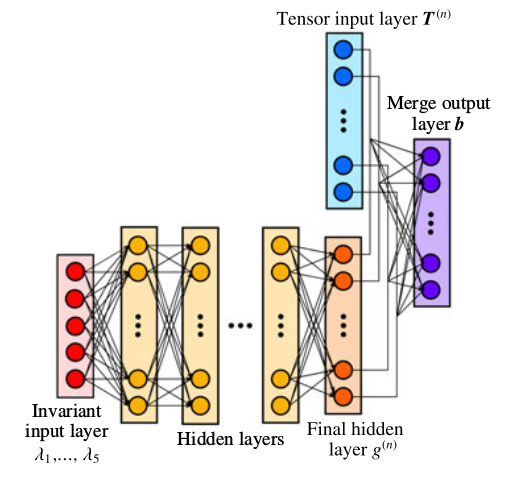
\includegraphics[scale=0.5]{TBNN.png}
\caption{Tensor embedded NN from \citep{kutz2017deep} et \citep{ling2016reynolds}}
\label{TBNN}
\end{figure}
 
\noindent \cite{pope1975more} propose de modifier l'hypothèse de Boussinesq qui consistait à écrire 
\begin{equation*}
\bar{u_i' u_j'} = \frac{2}{3} k \delta_{ij} - 2 \nu_t \bar{S_{ij}}
\end{equation*}
 Il propose plutôt de calculer 
\begin{equation*}
\frac{\bar{u_i' u_j'} }{2k}= \frac{1}{3} \delta_{ij} + \sum_\lambda G^\lambda T^\lambda_{ij} 
\end{equation*}
Avec une forme bien particulière pour $G$ et $T$. La première est une fonction des invariants du problème qui sont dans le cas tridimensionnel : 
\begin{equation*}
\mathbf{\Omega}= \left \{ \{\textbf{S}^2\}, \{\textbf{R}^2\}, \{\textbf{S}^3\}, \{\textbf{R}^2\textbf{S}\}, \{\textbf{R}^2 \textbf{S}^2\}\right \} 
\end{equation*}
La notation $\{ \}$ symbolise la trace du tenseur concerné. À noter, que l'invariant $\{\textbf{S}\}$ n'est pas utilisé directement (puisque nul) mais indirectement au travers l'utilisation du $\{\textbf{S}^3\}$. Également, les tenseurs considérés $\textbf{S}$ et $\textbf{R}$ sont définis par 
\begin{align*}
\textbf{S} &= \frac{k}{2\varepsilon}\left(\nabla_x\textbf{U} + \nabla^T_x\textbf{U} \right) \\[0.2cm]
\textbf{R} &= \frac{k}{2 \varepsilon}\left(\nabla_x\textbf{U} - \nabla^T_x\textbf{U} \right) 
\end{align*}

\noindent $T$ est composée de 10 tenseurs dans le cas tridimensionnel. Les 10 tenseurs proposés par \cite{pope1975more} et repris par \cite{ling2016reynolds} sont :
\begin{align*}
\textbf{T}^{(1)} &= \textbf{S} \\
\textbf{T}^{(2)} &= \textbf{S}\textbf{R} - \textbf{R}\textbf{S} \\
\textbf{T}^{(3)} &= \textbf{S}^2 - \dfrac{1}{3}\, \textbf{I} \cdot Tr \left( \textbf{S}^2 \right)\\
\textbf{T}^{(4)} &= \textbf{R}^2 - \frac{1}{3}\, \textbf{I} \cdot Tr \left( \textbf{R}^2 \right)\\
\textbf{T}^{(5)} &= \textbf{R}\textbf{S}^2 - \textbf{S}^2\textbf{R}\\
\textbf{T}^{(6)} &= \textbf{R}^2\textbf{S} + \textbf{S}^2\textbf{R} - \frac{2}{3}\, \textbf{I}\cdot Tr\left(\textbf{S}\textbf{R}^2 \right) \\
\textbf{T}^{(7)} &= \textbf{R}\textbf{S}\textbf{R}^2 - \textbf{R}^2\textbf{S}\textbf{R} \\
\textbf{T}^{(8)} &= \textbf{S}\textbf{R}\textbf{S}^2 - \textbf{S}^2\textbf{R}\textbf{S} \\
\textbf{T}^{(9)} &= \textbf{R}^2\textbf{S}^2 + \textbf{S}^2\textbf{R}^2 - \frac{2}{3}\, \textbf{I}\cdot Tr\left(\textbf{S}^2\textbf{R}^2 \right)\\
\textbf{T}^{(10)} &= \textbf{R}\textbf{S}^2\textbf{R}^2 - \textbf{R}^2\textbf{S}^2\textbf{R}
\end{align*}

\noindent Si $T$ peut être calculé en cours de processus, le calcul de $G$ reste encore obscur et justement les coefficients par rapport aux invariants sont définis par le training du NN utilisé ici avec 8 HL \footnote{La dernière HL en aura 10.}, 30 nœuds chacune et $learning\_rate = 2.5 \times 10^{-6}$. \\

Comme on peut le voir Fig.\eqref{TBNN}, les invariants sont injectés en entrée du réseau, suivent ensuite un processus classique propre au Feed-Forward NN. La dernière HL représentera les combinaisons linéaires de coefficients et de la base $\mathbf{\Omega}$. \\
L'output s'écrira alors : $$ b_{ij} = \sum_{n=1}^{10} g^{(n)}(\lambda_1,..,\lambda_5) T_{ij}^{(n)}$$
Ainsi on aura complètement reconstruit l'anisotropie que les solver RANS n'arrivent pas à etrouver, tout en s'assurant que ce tenseur vérifie bien les invariances Galiléennes. \\

Les RF donnent de bons résultats et sont en général plus rapide à entraîner. Seulement la construction d'Arbres de décision (DT) peut saturer l'utilisation de mémoire. En effet , \cite{ling2016machine} compare le temps de calcul et la mémoire utilisée pour les NN et les RF. La différence de temps de calcul (pour le training) est aussi marquant que la différence de mémoire utilisée. \\
On rapporte quelques données du tableau concernant la turbulence

\begin{table}[!h]
\centering
		% Table itself: here we have two columns which are centered and have lines to the left, right and in the middle: |c|c|
		\begin{tabular}{M{.45\textwidth} M{.3\textwidth} M{.2\textwidth} N}
		Algorithm & Compute time (CPU Hours) & \textbf{Memory usage }&\\[0.1cm]\hline
		Invariant \navy \textbf{RF} \bk / \red \textbf{NN} \bk & \navy 0.03 \bk / \red 7 \bk& \navy 0.4 \textbf{GB} \bk /  \red 0.1 \textbf{MB} \bk&\\[0.1cm]		
		Raw \navy \textbf{RF} \bk / \red \textbf{NN} \bk 10 rotations 2D & \navy 0.3 \bk / \red 105 \bk& \navy 0.9 \textbf{GB} \bk /  \red 2 \textbf{MB} \bk&\\[0.1cm]
		Raw \navy \textbf{RF}\bk / \red \textbf{NN} \bk 10 rotations 3D & \navy 46 \bk / \red 1176 \bk& \navy 13 \textbf{GB} \bk / \red 2 \textbf{MB} \bk&\\[0.1cm]\hline
		\end{tabular}
		\caption{\footnotesize Comparaisons des temps de calcul et de mémoire mobilisée pour les algo Random Forest et Neural Network. On compare également ces deux algos avec des entrées différentes : les invariants dans un premier temps puis les valeurs de toutes les composantes \textbf{S} et \textbf{R}. On rajoute ces mêmes entrées après les avoir multipliées par des matrices de $\mathcal{SO}(3)$}
\end{table}


\pagebreak

\bibliographystyle{apalike}
\bibliography{bibliotheque}

\end{document}